\subsection{Effect Of Aggregating Sectoral Data\label{sec: minormajor}}

Aggregating the economy into coarser sector classifications washes out the reallocation effect. The left panel in figure \ref{fig:minormajor} plots the cumulative Haltiwanger decomposition using the `payroll labour share' approach and uses data from 60 sectors defined at the NAICS 3-digit level. There is a positive reallocation effect. The decomposition in the right panel in figure \ref{fig:minormajor} uses weights and labour shares aggregated into ten NAICS 2-digit industries. Both the between-sector and cross terms disappear - the Between and Cross lines are flat - even though reallocation is quantitatively important at the 3-digit classification level. The reason is that between-sector reallocation between any two NAICS 3-digit industries will always be counted as a within-sector contribution at the NAICS 2-digit level when the 3-digit industries are in the same 2-digit classification. Aggregating the economy into coarser definitions loads onto the within-sector contribution. I attempt to nullify the issue by using the most disaggregated data possible for each labour share definition. 

\begin{figure}[h]
  \centering
  \caption{\normalsize Between-sector effect disappears when aggregating NAICS 3-digit to NAICS 2-digit}
\subfloat[NAICS 3-digit sectors]{\label{fig:elsby_hw}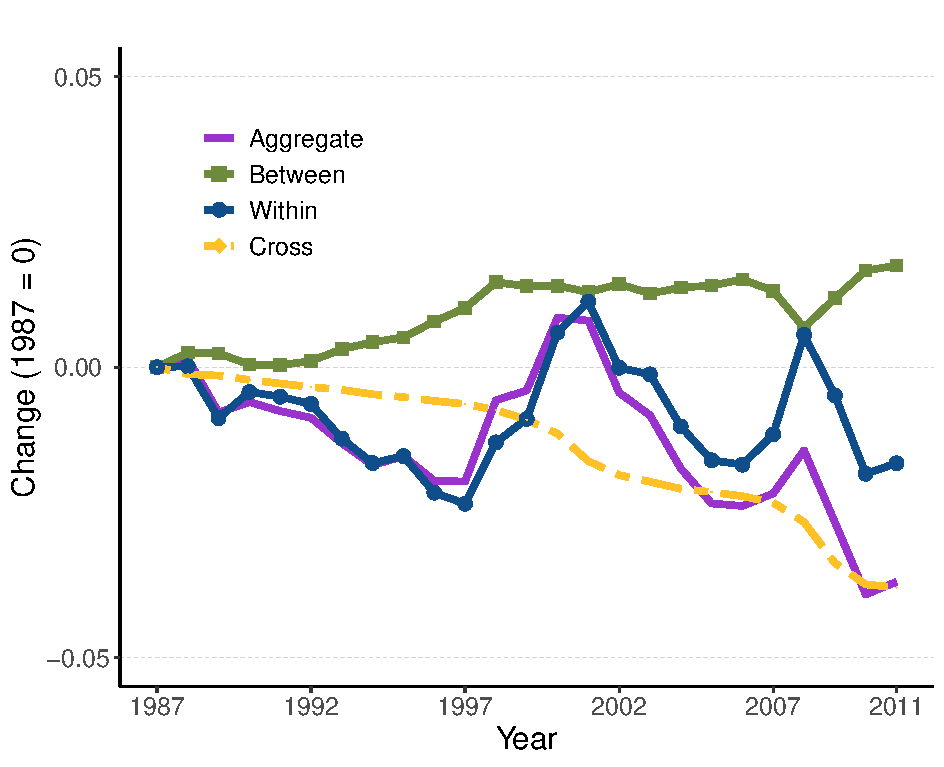
\includegraphics[width=.45\linewidth]{Appendix/Figures/elsby_hw_D_graph.pdf}}
\subfloat[NAICS 2-digit sectors]{\label{fig:elsby_hw}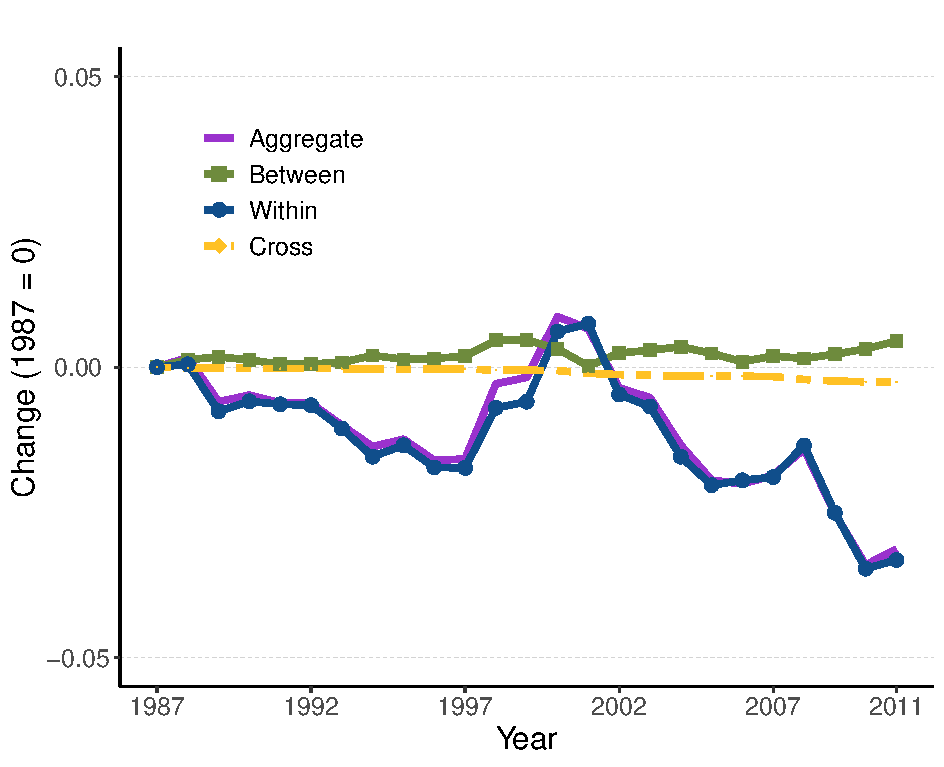
\includegraphics[width=.45\linewidth]{Appendix/Figures/elsby_hw_D_MINOR_MAJOR_graph.pdf}}\vfill
\begin{minipage}{\linewidth}
\captionsetup{justification=raggedright,singlelinecheck=false}
    \caption*{\textit{Notes}: Cumulative between, within, cross terms for the Haltiwanger method using the payroll labour share. The left panel uses data at the NAICS 3-digit level (60 sectors) and the right panel uses the same data but aggregated into NAICS 2-digit level (10 sectors). `0.05' on the y-axis corresponds to 5 percentage points (pp). \\
    \textit{Source}: BEA and the \citet{elsbyDeclineLaborShare2013a} replication package.}
\end{minipage}
\label{fig:minormajor}
\end{figure}